\subsection{Использование АР для детектирования ШПС}
Известно, что АР подход широко применяется в детектировании и кодировании голоса и видео, в восстановлении сигналов и т.д.
Более точно - АР-модели целесообразно применять для получения спектров с острыми пиками, но без глубоких впадин (нулей).
Так же в пользу выбора АР-модели может быть принят тот факт, что часто вычислительные затраты для оценивания АР-модели 
ниже чем вычислительные затраты требуемые для оценки параметров СС- и АРСС моделей \cite{marpl_book}.

Специфичной для детектирования ШПС является необходимость определения точной фазы ПСП
для работы с сигналом. Так же при обработке ШПС от нескольких источников с разными ПСП необходимо учитывать,
что оценка спектра будет смещенной и требуется его корректировка.

\subsubsection{Детектирование ШПС от одного источника}

Рассмотрим применение данного подхода для детектирования одного сигнала ШПС. Схема алгоритма представлена на рисунке \ref{pic:lpc_basic}.
\begin{figure}[H]
	\center\scalebox{0.8}{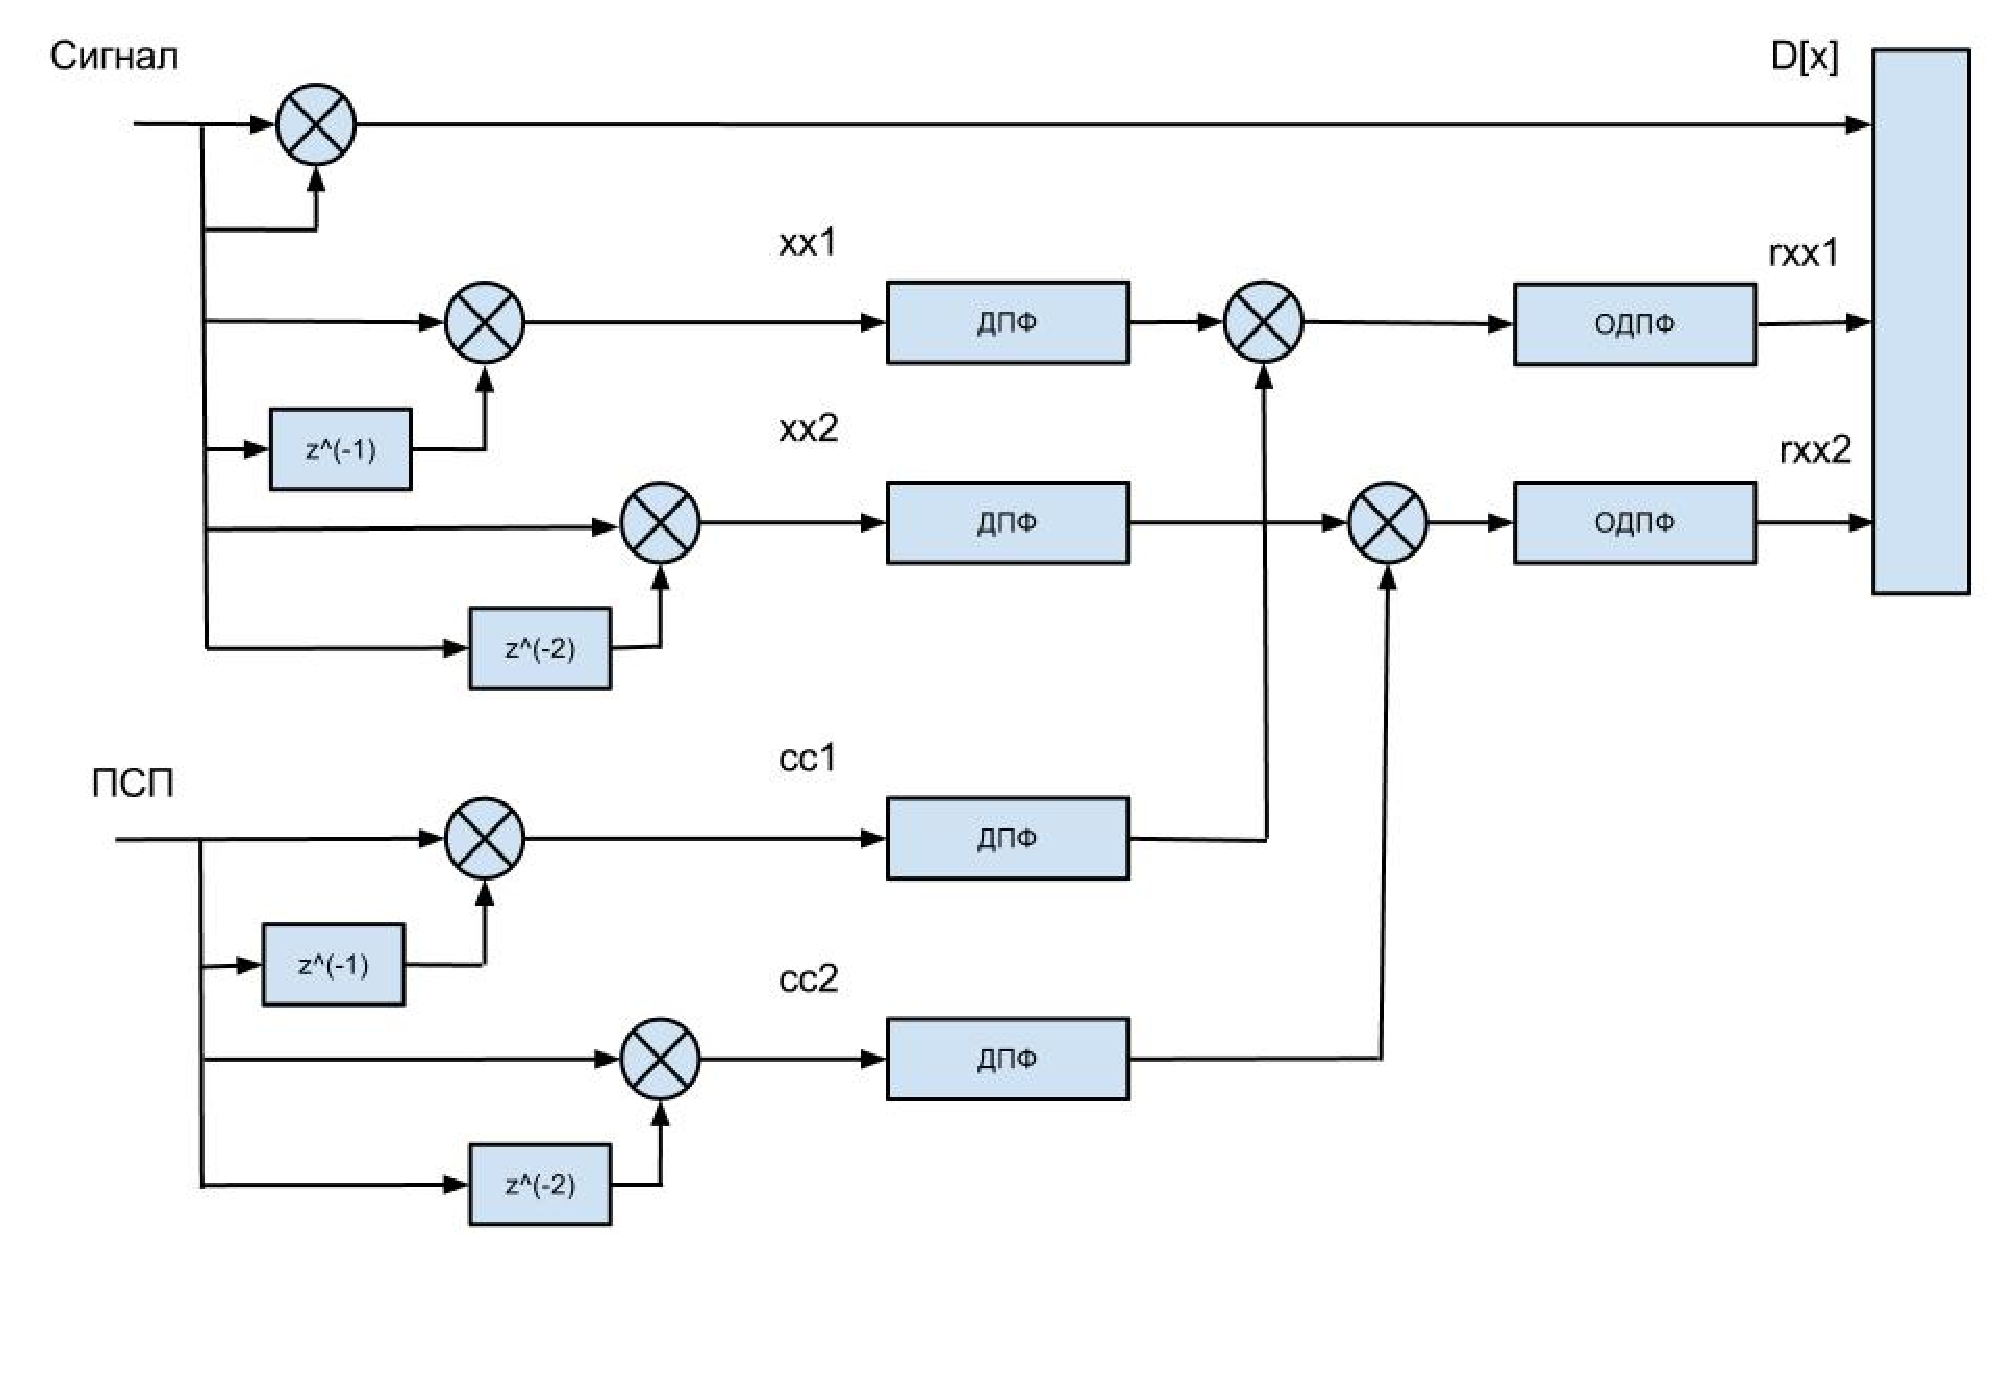
\includegraphics[width=1\linewidth]{lpc.eps}}
	\caption{Общая схема применения АР модели для детектирования ШПС сигнала}
	\label{pic:lpc_basic}
\end{figure}
Так как нам необходимо подобрать фазу ПСП мы пользуемся БПФ для отыскания всех позиций кода (глава \ref{sec1_fft}).

\begin{figure}[H]
	\center\scalebox{1}{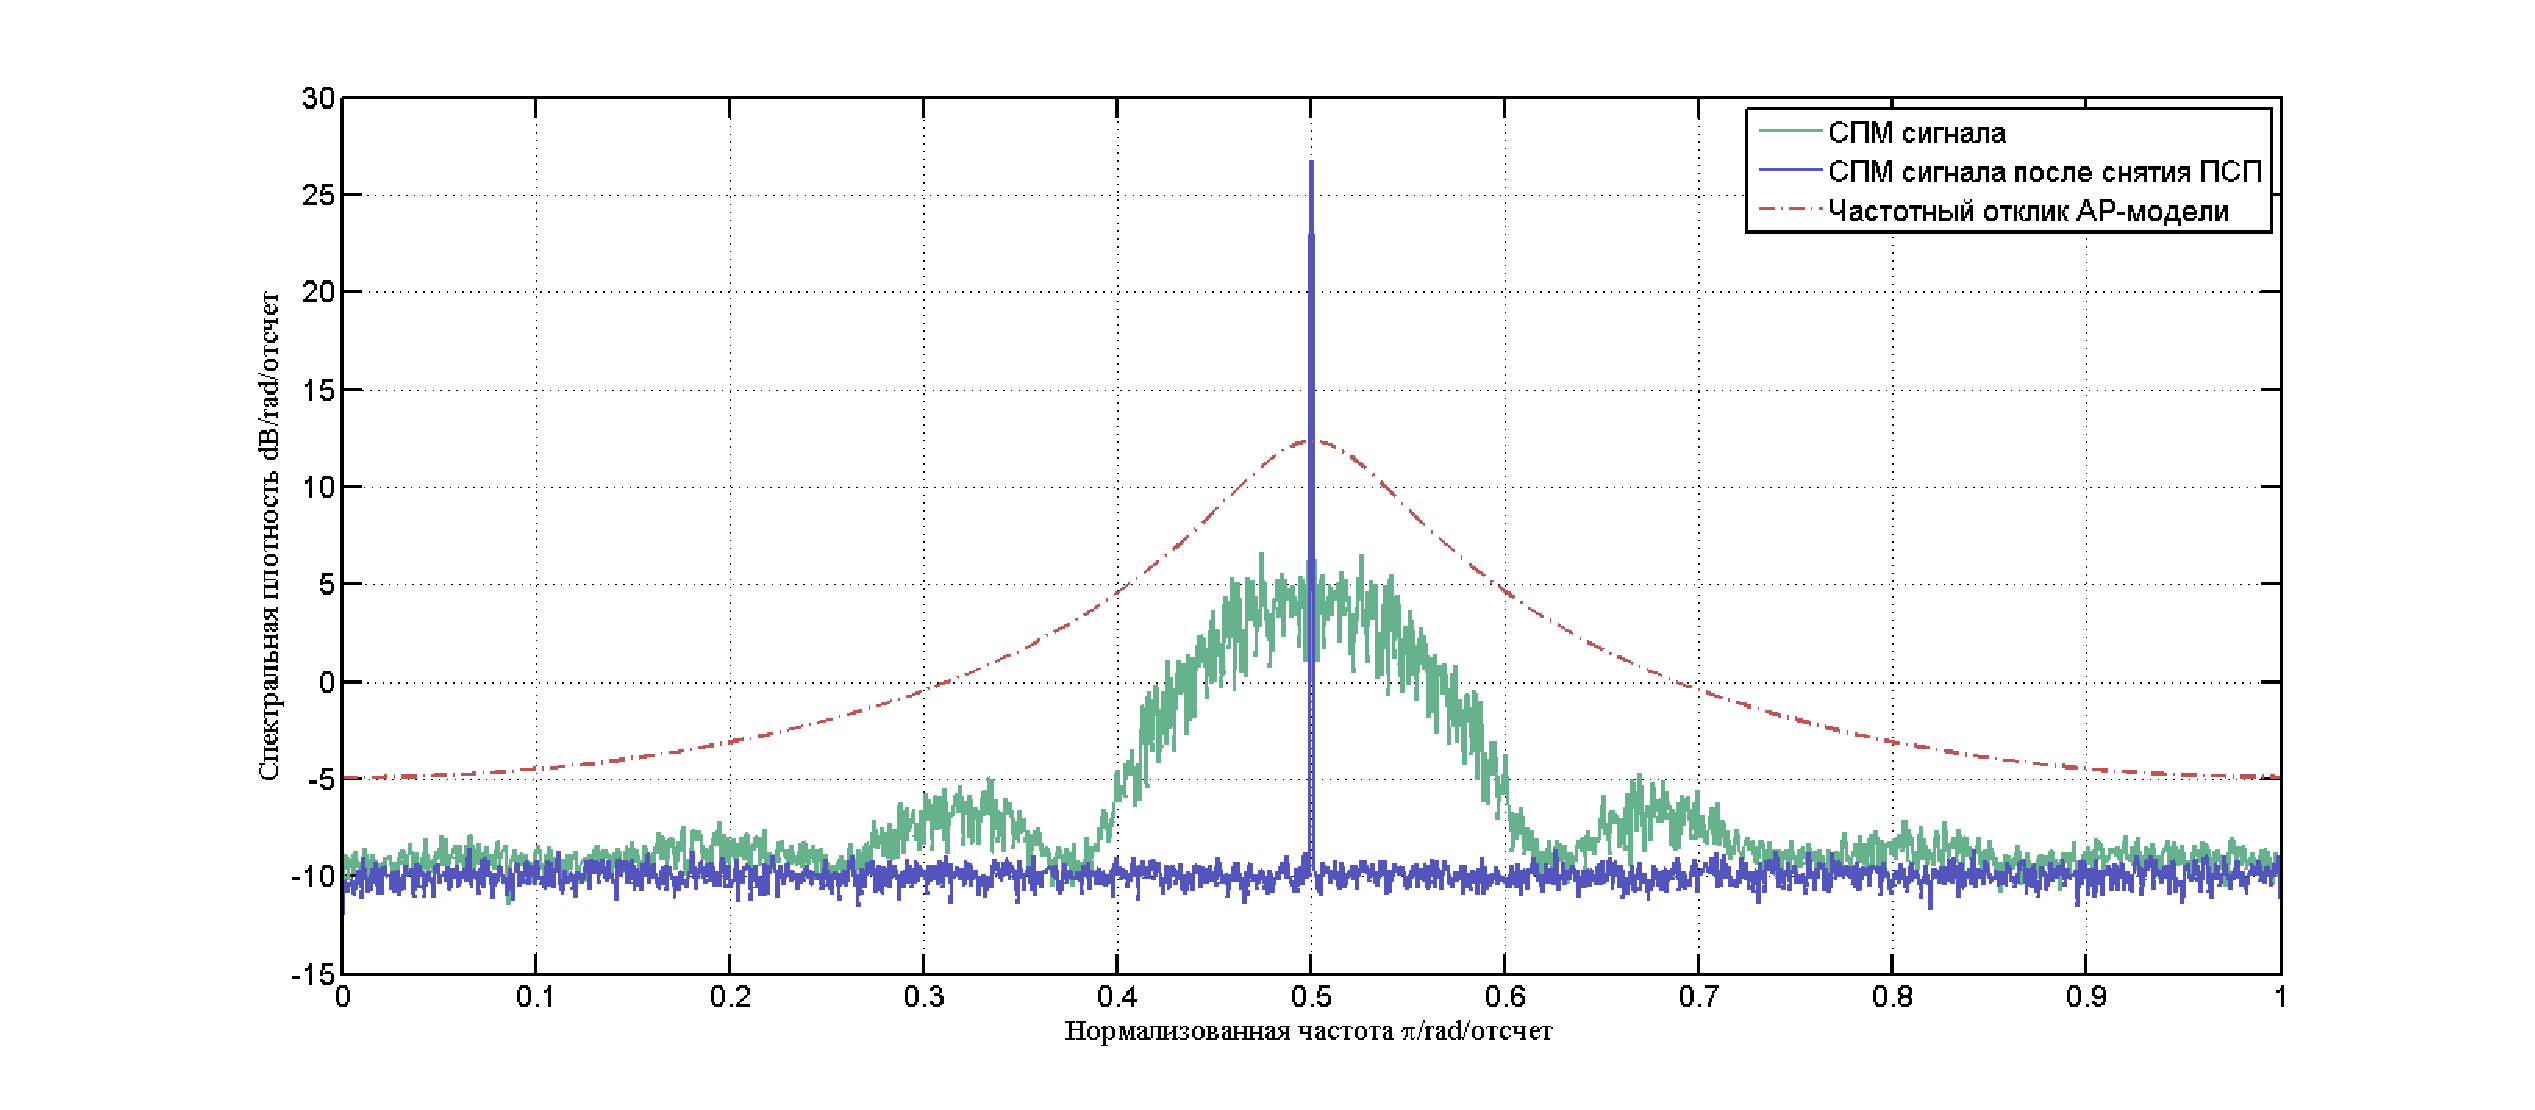
\includegraphics[width=1\linewidth]{lpc_1sat.eps}}
	\caption{Общая схема применения АР модели для детектирования ШПС сигнала}
	\label{pic:lpc_1sat}
\end{figure}

\begin{figure}[H]
	\center\scalebox{1}{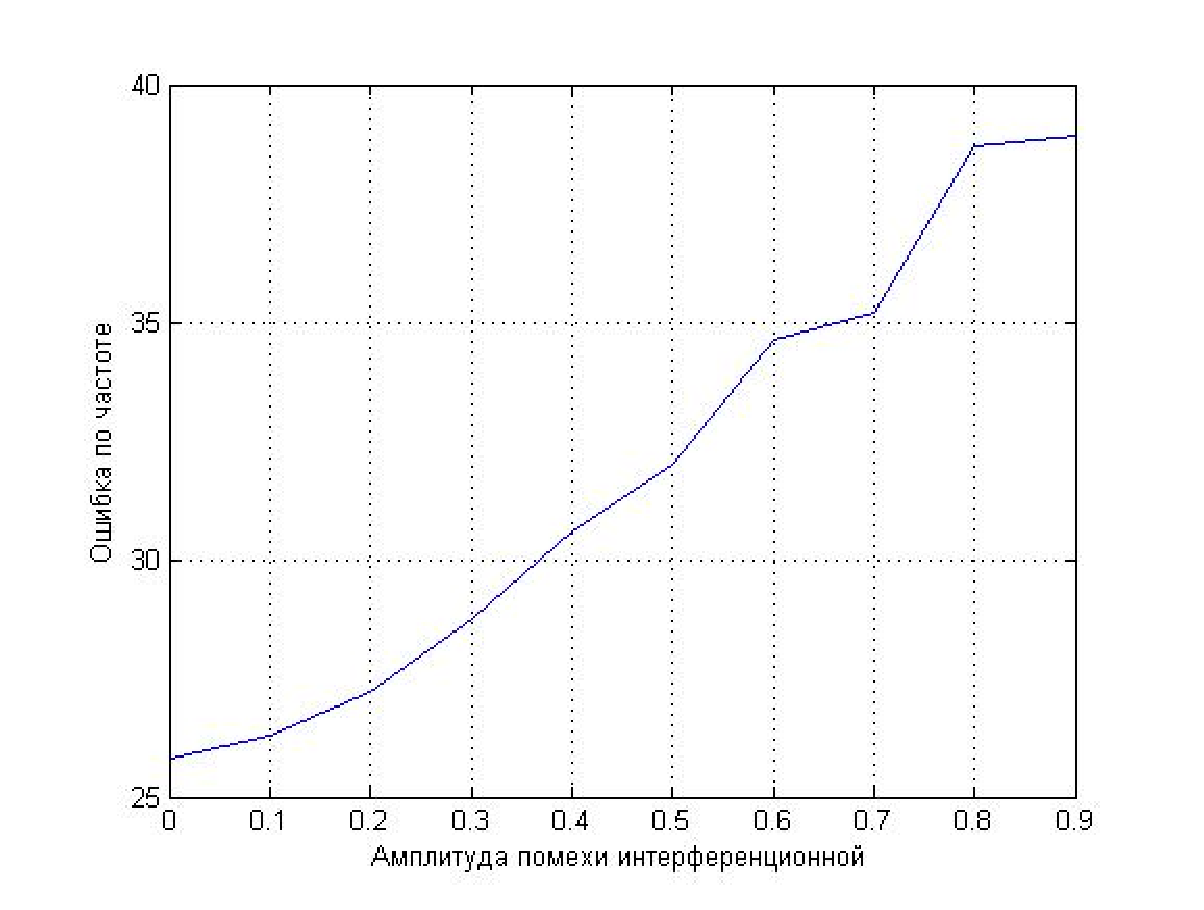
\includegraphics[width=1\linewidth]{lpc_interference.eps}}
	\caption{Зависимость ошибки оценки пика от энергии интерференционной помехи}
	\label{pic:lpc_1sat}
\end{figure}

\newpage
